%
% $RCSfile: chain_of_responsibility.tex,v $
%
% Copyright (c) 2004. Christian Heller. All rights reserved.
%
% No copying, altering, distribution or any other actions concerning this
% document, except after explicit permission by the author!
% At some later point in time, this document is planned to be put under
% the GNU FDL license. For now, _everything_ is _restricted_ by the author.
%
% http://www.cybop.net
% - Cybernetics Oriented Programming -
%
% http://www.resmedicinae.org
% - Information in Medicine -
%
% @author Christian Heller <christian.heller@tuxtax.de>
%

\paragraph{Chain of Responsibility}
\label{chain_of_responsibility_heading}

The \emph{Chain of Responsibility} pattern \cite{gamma1995} is similar to the
\emph{Composite}, in that it represents a recursive structure as well. Objects
destined to solve a task are linked with a corresponding \emph{Successor}
(figure \ref{chain_figure}), such forming a chain. If an object is not able to
solve a task, that task is forwarded to the object's successor, along the chain.

\begin{figure}[ht]
    \begin{center}
        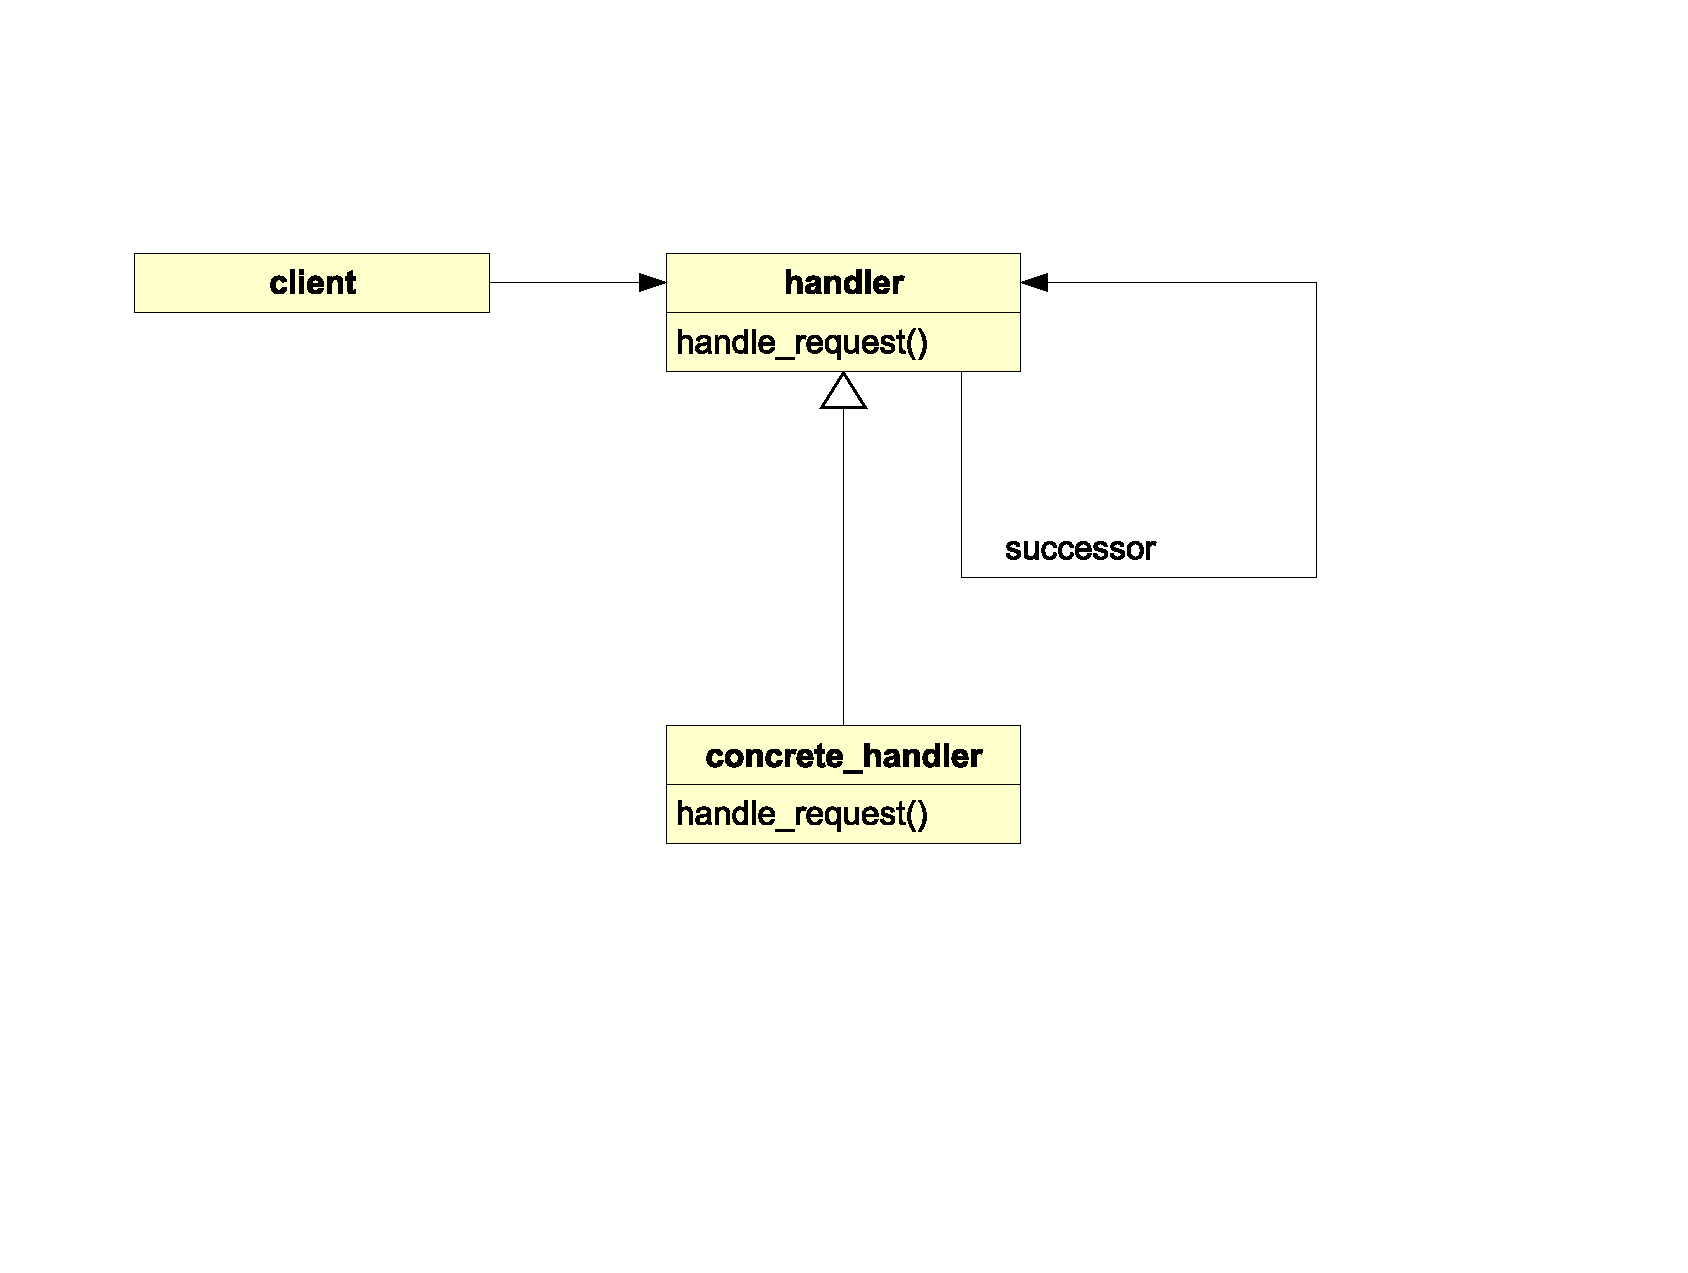
\includegraphics[scale=0.3]{vector/chain.eps}
        \caption{Chain of Responsibility Pattern}
        \label{chain_figure}
    \end{center}
\end{figure}

The pattern found wide application, for example in help systems, in event
handling frameworks or for exception handling. Its \emph{Handler} class is
known under synonyms like \emph{Event Handler}, \emph{Bureaucrat} or
\emph{Responder}.

Frequently, the pattern gets misused by delegating messages not only to children
but also to the parent of objects. The \emph{Hierarhical Model View Controller}
(HMVC) pattern is one example for this. It causes unfavourable bidirectional
dependencies (section \ref{bidirectional_dependency_heading}) and leads to
stronger coupling between the layers of a framework, because parent- and child
objects then reference each other.
